% !TEX root = thesis.tex

\documentclass[thesis.tex]{subfiles}

\begin{document}

\chapter{Camera Module}
\label{appendix:camera-module}

The camera module photographed from the top and side. Cardboard is used to encase the taggant and cover it from ambient lighting. an additional piece of cardboard is used to set the smartphone to be at a fixed distance (of lens MFD) from the taggant allowing more accurate focus.

\begin{figure}[h]
\centering 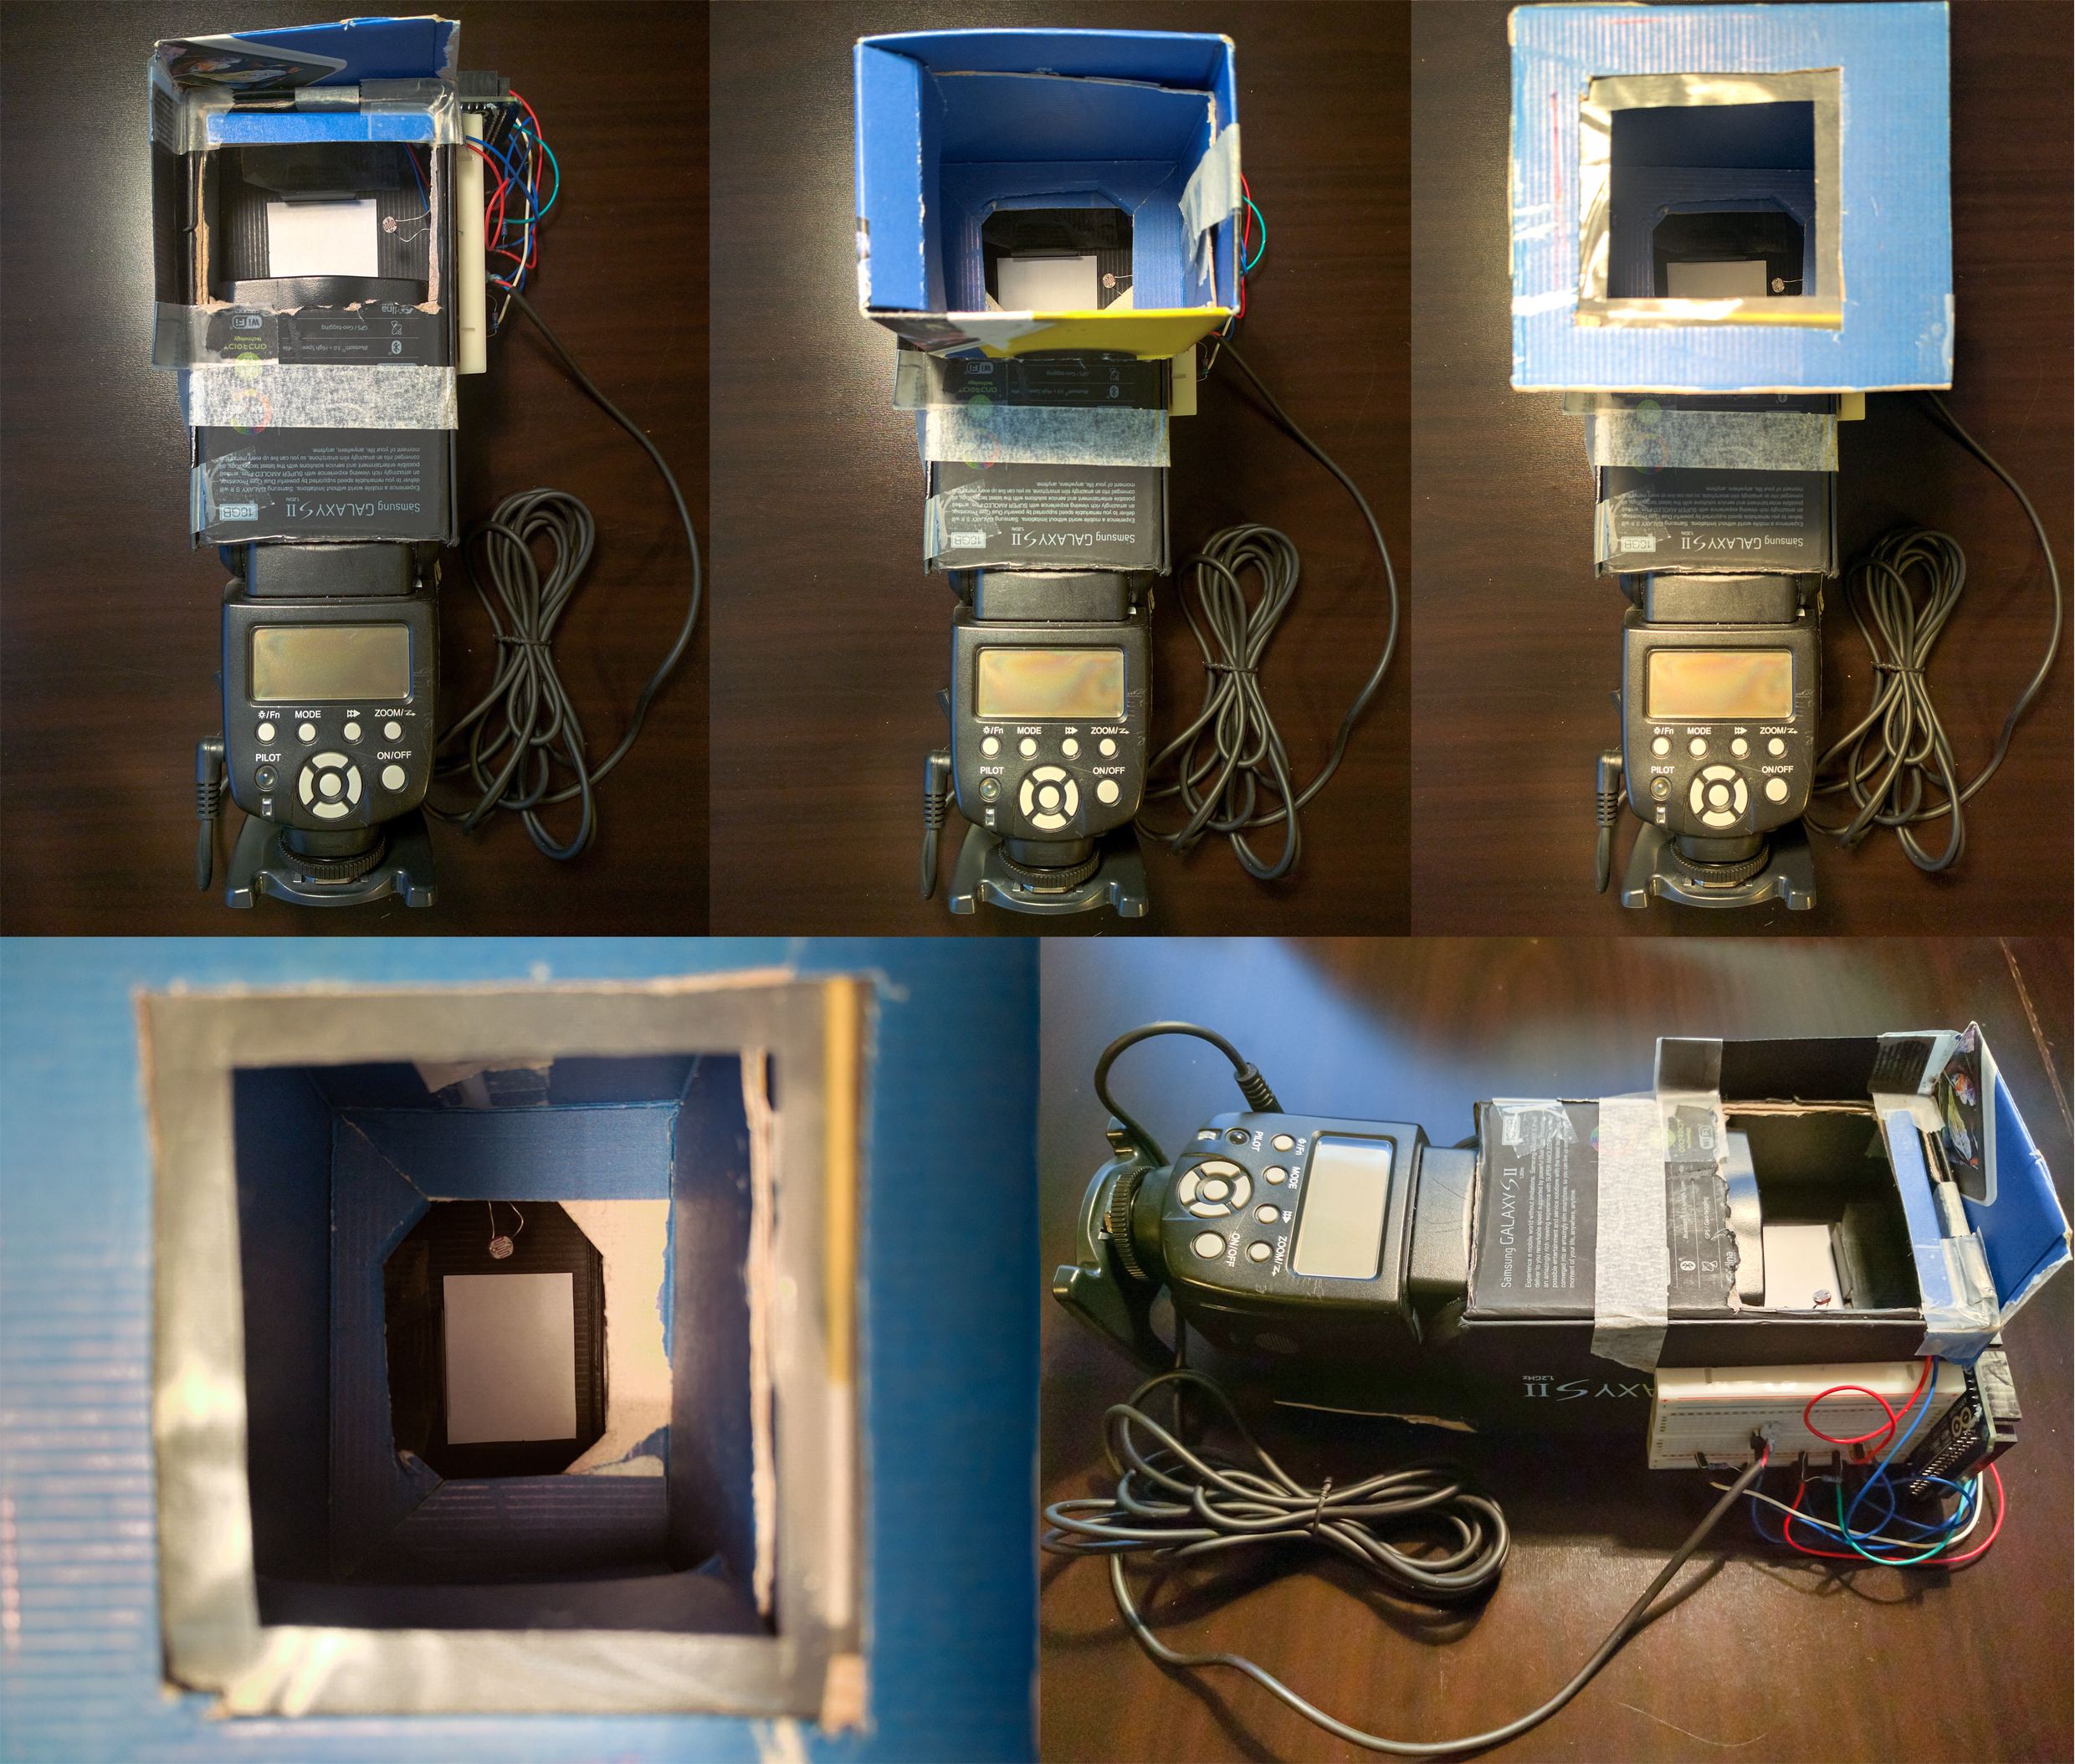
\includegraphics[width=\textwidth,height=\textheight,keepaspectratio=true]{images/design_implementation/camera_module-actual.jpg}
\end{figure}




\chapter{Microcontroller Schematics}
\label{appendix:camera-module-schematics}

The schematics for the external camera module featuring an Arduino Mega 2560 microcontroller. an optocoupler (4N35) is used to safely isolate the external light source from the rest of the circuit.

\begin{figure}[h]
\centering 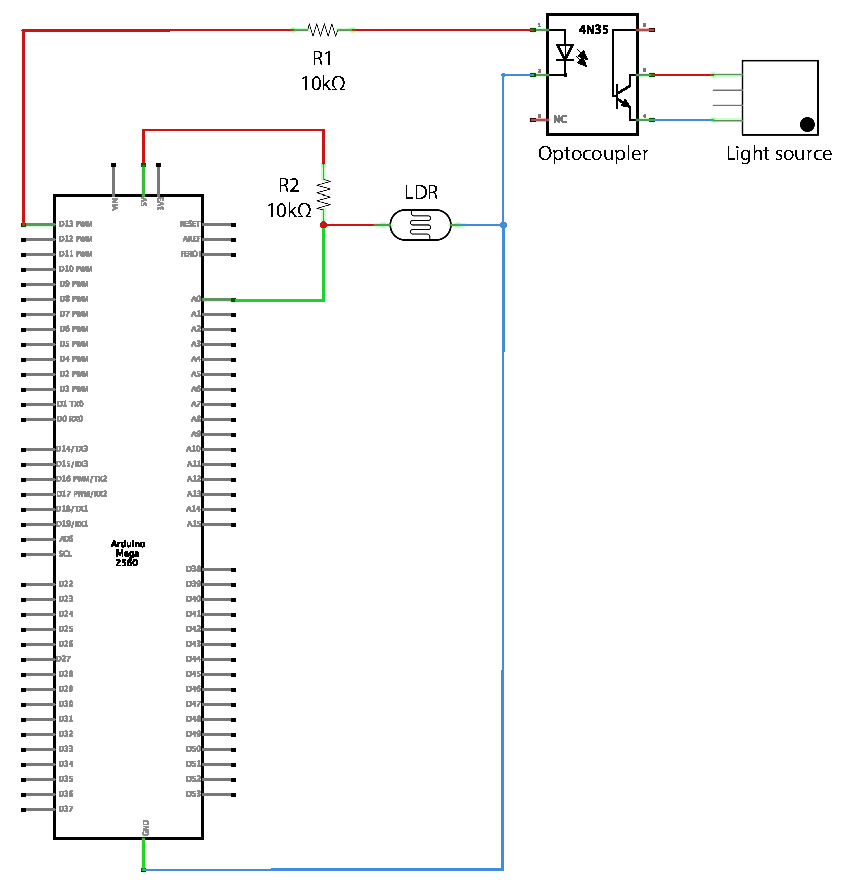
\includegraphics[width=12cm]{images/design_implementation/arduino_schematics.pdf}
\end{figure}





\chapter{Microcontroller Program (Arduino)}
\label{appendix:microcontroller-program}

The code utilizes Simon Monk's Arduino Timer library (version 1.3) \cite{arduino_timer_library}.

\lstinputlisting[language=C++,caption={main.ino}]{../app/camera-module/arduino/code/code.ino}
\clearpage
\lstinputlisting[language=C++,caption={is\_focused.ino}]{../app/camera-module/arduino/code/is_focused.ino}




\chapter{Fingerprint format}
\label{appendix:fingerprint}

The fingerprint can be represented as a $n \times m$ matrix where $n$ denotes the number of frames and $m$ the maximum number of peaks found in a single frame (sample), and encoded as a JavaScript array with additional metadata:
\[
M=
  \begin{bmatrix}
    P_{11} & P_{12} & P_{13} \\
    P_{21} & P_{22} & 0 \\
    P_{31} & 0 & 0
  \end{bmatrix}
\]
\begin{lstlisting}[language=json,firstnumber=1]
[
  {
    timestamp: 252,
    peaks: [
      { hue: 76, intensity: 770 },
      { hue: 90, intensity: 693 },
      { hue: 60, intensity: 301 }
    ]
  },
  {
    timestamp: 844,
    peaks: [
      { hue: 74, intensity: 672 },
      { hue: 60, intensity: 310 }
    ]
  },
  {
    timestamp: 1440,
    peaks: [
      { hue: 60, intensity: 466 },
      { hue: 71, intensity: 466 }
    ]
  }
]
\end{lstlisting}


\chapter{Fingerprint Design Document}
\label{appendix:fingerprint-design-doc}
A CouchDB design document used for creating an index keyed by the peak count and weighted hue average of the first sample of each fingerprint to allow fingerprints to be queried directly by peak count and average hue.
\vspace{5mm}

\lstinputlisting[language=JavaScript]{./chapters/design_doc.js}

\chapter{Experiment Taggants}
\label{appendix:taggants}
\enlargethispage{10\baselineskip}
For each LumiNova\textregistered\ pigment (luminophore) a stock solution was created. The taggants were created by pipeting the stock solutions in increments of $50\mu l$ into intermediary solutions, from which another $50\mu l$ would be pipeted onto a blank white carton as the taggant. For example, taggant \emph{13VP} would require $200\mu l$ of stock solution ($50\mu l$ and $150\mu l$ of pigments G and O, respectively), of which $50\mu l$ would eventually be pipeted on to the carton. In total, 16 different taggants were prepared for the experiement (including two samples for each taggant): \emph{S}, \emph{P}, \emph{13SP}, \emph{13SV}, \emph{13VP}, \emph{24SP}, \emph{24SV} and \emph{24VP}.

\vspace{-1em}
\begin{table}[ht]
  \caption{The stock solutions used for preparing the taggants were created by mixing phosphor and a transparent carrier together.}

  \begin{center}
  \begin{tabular}{| m{1.75cm} | c | c |}
    \hline
    \textbf{Pigment}  & \textbf{Phosphor (g)} & \textbf{Transparent carrier (ml)} \\ \hline
    O & 0,1416 & 1,42 \\
    \hline
    G & 0,1558 & 1,56 \\
    \hline
    DB & 0,1454 & 1,45 \\
    \hline
  \end{tabular}
  \end{center}
\end{table}
\vspace{-2.75em}
\begin{table}[ht]
  \caption{The experiment taggants and their pigment proportions. The numbers indicate how many $50\mu l$ of each stock solution was used per taggant.}

  \begin{center}
  \begin{tabular}{| m{1.75cm} | c | c | c |}
    \hline
    \textbf{Taggant}  & \textbf{Red (O)} & \textbf{Green (G)} & \textbf{Blue (DB)} \\ \hline
    S & -- & -- & 1 \\
    \hline
    P & 1 & -- & -- \\
    \hline
    13SP & 3 & -- & 1 \\
    \hline
    13VP & 3 & 1 & -- \\
    \hline
    13SV & -- & 3 & 1 \\
    \hline
    24SP & 4 & -- & 2 \\
    \hline
    24VP  & 4 & 2 & -- \\
    \hline
    24SV & -- & 4 & 2 \\
    \hline
  \end{tabular}
  \end{center}
\end{table}

\chapter{Capture Presets}
\label{appendix:capture-presets}

Nine different capture presets were used to capture the taggants: six presets for the Samsung S4 ($an$) and three presets for the Lumia 1020 ($wp$). The number of frames, delay, White Balance and ISO were given a fixed value. A description of the parameters listed below is provided to Table \ref{table:camera-parameters}.

\begin{table}[ht]
  \caption{The capture presets and corresponding parameter values. Each row represents a preset.}

  \begin{center}
  \begin{tabular}{| c | c | c | c | c |}
    \hline
    \textbf{Preset} & \textbf{Focus Distance} & \textbf{Torch} & \textbf{Resolution (px)} & \textbf{Interval (ms)} \\ \hline
    $an_{200}$ & Macro & No & $1280\times720$ & 200 \\
    \hline
    $an_{400}$ & Macro & No & $1280\times720$ & 400 \\
    \hline
    $an_{600}$ & Macro & No & $1280\times720$ & 600 \\
    \hline
    $an_{200r}$ & Macro & No & $1920\times1080$ & 200 \\
    \hline
    $an_{400r}$ & Macro & No & $1920\times1080$ & 400 \\
    \hline
    $an_{600r}$ & Macro & No & $1920\times1080$ & 600 \\
    \hline
    $wp_{200}$ & Fixed minimum & Yes & $1280\times720$ & 200 \\
    \hline
    $wp_{400}$ & Fixed minimum & Yes & $1280\times720$ & 400 \\
    \hline
    $wp_{600}$ & Fixed minimum & Yes & $1280\times720$ & 600 \\
    \hline
  \end{tabular}
  \end{center}
\end{table}

\begin{table}[ht]
  \caption{Camera parameters that were given a fixed value}

  \begin{center}
  \begin{tabular}{| c | c | c | c |}
    \hline
    \textbf{Frames}  & \textbf{Delay (ms)} & \textbf{White Balance} & \textbf{ISO} \\ \hline
    5 & 250 & Daylight & Auto \\
    \hline
  \end{tabular}
  \end{center}
\end{table}

\end{document}